\documentclass{standalone}
\usepackage{tikz,amsmath}
\tikzset{ block/.style = {draw, fill=white, very thick, rectangle, minimum height=1cm, minimum width=2cm},}
\tikzset{sum/.style= {draw, fill=white, very thick, circle, node distance=1cm},}
\begin{document}
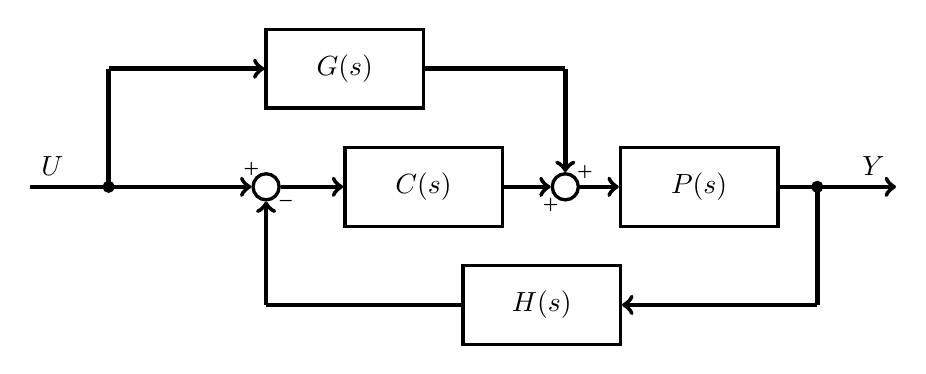
\begin{tikzpicture}[scale=2]
    \node[sum](sum)at(-1,0){};
    \draw[->,ultra thick](-1.5,0)--(sum.180)node[above]{$\scriptscriptstyle\boldsymbol{+}$};
    \filldraw[black](-2,0)circle(1pt);
    \draw[-,ultra thick](-2.5,0)node[above right]{$U$}--(-1.5,0);
    \node[block, right of=sum, node distance=2cm](c){$C(s)$};
    \node[sum]at(0.9,0)(sum2){};

    
    \draw[-,ultra thick](-2,0)--(-2,0.75);
    \node[block]at(-0.5,0.75)(g){$G(s)$};
    \draw[->,ultra thick](-2,0.75)--(g.180);
    \draw[-,ultra thick](g.0)--(0.9,0.75);
    \draw[->,ultra thick](0.9,0.75)--(sum2.90)node[right]{$\scriptscriptstyle\boldsymbol{+}$};



    \draw[->,ultra thick](sum.0)--(c.180);
    \filldraw[black](2.5,0)circle(1pt);

    \draw[->,ultra thick](2.5,0)--(3,0)node[above left]{$Y$};
    \draw[-,ultra thick](2.5,-0.75)--(2.5,0);

    \node[block]at(0.75,-0.75)(h){$H(s)$};
    \node[block]at(1.75,0)(p){$P(s)$};

    \draw[-,ultra thick](p.0)--(2.5,0);
    \draw[->,ultra thick](c.0)--(sum2.180)node[below]{$\scriptscriptstyle\boldsymbol{+}$};
    \draw[->,ultra thick](sum2.0)--(p.180);

    \draw[->,ultra thick](2.5,-0.75)--(h.0);
    \draw[-,ultra thick](h.180)--(-1,-0.75);
    %\draw[-,ultra thick](2.5,-0.75)--(-1,-0.75);
    \draw[->,ultra thick](-1,-0.75)--(sum.270)node[right]{$\scriptscriptstyle\boldsymbol{-}$};
\end{tikzpicture}
\end{document}